\chapter{Constructing Interpretive Features}\label{chap:features}

After collecting the data and carefully defining the problem, we started constructing sophisticated interpretive features (aka \cov) hypothesized to be predictive of \sti. As previously mentioned, we split the course into 15 time slices (weeks). Thus, for each defined feature, we assign each student a feature-value each week. For example, each student has a value for the feature ‘\sti’ for each of the 15 weeks. The value is 0 if the student has already stopped out by not submitting any more assignments, or it is 1 if the student will submit assignments in the future.

\section{Feature origins}

With the database, we then proceeded to write the scripts to extract the \cov for our model. By analyzing the \cov we aimed to capture behavioral patterns that could be indicative of loss of interest or loss of motivation among several others. We approached this in three different ways:

\begin{itemize}
\item We brainstormed feature ideas as researchers. Next, we implemented our own ideas by writing feature extraction scripts. We call these features \selfself.
\item We asked others for ideas of what might be predictive of \sti. The people we asked included students, teachers and external researchers. We refer to this group collectively as `the crowd.' We identified ideas that we had not implemented yet, and constructed feature extraction scripts ourselves. We call these \crowdself.
\item Finally, we asked `the crowd' to brainstorm predictive features, and to send us feature extraction scripts that we could run on MOOCdb. We provided people with a mock dataset with an identical data schema. Thus, instead of providing actual student data, we empowered the crowd to join in our data science efforts. We call the resulting features \crowdcrowd.
\end{itemize}


\subsection{\selfself}
Table \ref{table:self_proposed_self_extracted} summarizes the features we brainstormed and extracted. Each feature is calculated on a per student, per week basis. A * indicates that a disambiguating explanation follows underneath.

\begin{table*}[htp]
	\centering
	\caption{List of \selfself \cov}\label{table:self_proposed_self_extracted}
{
		\begin{tabular}{|c|p{4cm}|p{10cm}|}
			\hline
							& Name 													& Definition																									 \\ \hline
			\x{1}		& stopout 											& Whether the student has stopped out or not 									\\ \hline
			*\x{2}	& total duration								& Total time spent on all resources														\\ \hline
			\x{3}		& number forum posts						& Number of forum posts																				\\ \hline
			\x{4}		& number wiki edits							& Number of wiki edits																				\\ \hline
			*\x{5}	& average length forum post			& Average length of forum posts																\\ \hline 
			*\x{6}		& number distinct problems submitted	& Number of distinct problems attempted 							\\ \hline 
			*\x{7}	& number submissions						& Number of submissions \footnote{In our terminology, a submission corresponds to a problem attempt. In 6.002x, students could submit multiple times to a single problem. We therefore differentiate between problems and submissions.}																				\\ \hline
			\x{8}		& number distinct problems correct & Number of distinct correct problems 											\\ \hline 
			\x{9}	& average number submissions					& Average number of submissions per problem (\x{7} / \x{6})			\\ \hline 
			\x{10} & observed event duration per correct problem		& Ratio of total time spent to number of distinct correct problems (\x{2} / \x{8}). This is the inverse of the percent of problems correct \\ \hline 
			\x{11} & submissions per correct problem		& Ratio of number of problems attempted to number of distinct correct problems	(\x{6} / \x{8})	\\ \hline
			\x{12} & average time to solve problem	& Average time between first and last problem submissions for each problem (average(max(submission.timestamp) - min(submission.timestamp) for each problem in a week) )															\\ \hline
			*\x{13} & observed event variance			& Variance of a student's observed event timestamps  					 \\ \hline
			\x{14} & number collaborations				& Total number of collaborations	(\x{3} + \x{4})														 \\ \hline
			\x{15} & max observed event duration	& Duration of longest observed event													 \\ \hline
			*\x{16} & total lecture duration				& Total time spent on lecture resources 											\\ \hline
			*\x{17} & total book duration					& Total time spent on book resources													 \\ \hline
			*\x{18} & total wiki duration					& Total time spent on wiki resources													 \\ \hline
		\end{tabular}
	}
\end{table*}

\begin{itemize}

\item \x{2}, \x{16}, \x{17}, \x{18}: These features are based on observed event duration. The edX server logs did not explicitly provide this, so we need to infer the duration based on the timestamps of the start of observed events. We assume that a student observed an event until he observed a different event (a new timestamp). This is a similar approach used by industry web-profile metrics. Sometimes, the spacing between observed events is very large, presumably because the user stopped interacting with the website. This is handled by setting the last observed event's duration to a MAX\_DURATION. For example, if Student A had three observed events with timestamps, T1, T2 and T3, the duration of the first event would be T2 - T1, the duration of the second is T3 - T2, and the duration of the third is MAX\_DURATION, since there is no T4. Additionally if $T3 - T2 > 60$, the duration is set to MAX\_DURATION. In our case, we set MAX\_DURATION to be 60 minutes, because our data included durations of up to $\sim$ 60 minutes.

\item \x5: A forum post's length is the number of characters in the forum post (i.e. the length of the string). We used MySQL's length function.

\item \x6, \x7: With problem submissions, week number is ambiguous. Students may submit a problem at any time (assuming the problem is released), regardless of when the problem is due. In other words, even if a problem corresponds to week number 3, a student could submit that problem in week 5. For these features, we counted a submission in week w1 if the submission's timestamp is in w1, regardless of whether or not the problem is part of w1's assigned content.  We chose to do this because the feature is meant to capture a student's weekly activity.

\item \x{13}: For this feature, we tried to measure the consistency of a student's observed event patterns relative to the time of day (i.e., a student who always works on the course at 7:00 a.m. would have small variance for that week). To capture event variance, for each day, we counted the number of seconds after midnight of the observed event timestamp. We created a distribution of all of the number of seconds for each student each week. Then, we calculated the variance of the distribution (each student, week pair has it's own distribution). This variance becomes the feature. Note: student's participate from around the world, but the timestamp is in UTC time. However, because variance is valued over absolute value, the actual time is irrelevant. 

\end{itemize}

\subsection{\crowdself}\label{section:crowdself}
Table \ref{table:crowd_proposed_self_extracted} summarizes the features the crowd hypothesized, but we extracted. Each feature is calculated on a per student, per week basis. A * indicates that a disambiguating explanation follows underneath.

\begin{table*}[htp]
	\centering
	\caption{List of \crowdself \cov}\label{table:crowd_proposed_self_extracted}
{
		\begin{tabular}{|c|p{4cm}|p{10cm}|}
			\hline
							& Name 													& Definition																									 \\ \hline
			$x_{201}$ & number forum responses			& Number of forum responses																		\\ \hline
			*$x_{202}$ & average number of submissions percentile	& A student's average number of submissions (feature 9) as compared with other students that week as a percentile				\\ \hline
			*$x_{203}$ & average number of submissions percent	& A student's average number of submissions (feature 9) as a percent of the maximum average number of submissions that week																																			\\ \hline
			*$x_{204}$ & pset grade										& Number of the week's homework problems answered correctly / number of that week's homework problems																																												\\ \hline
			$x_{205}$ & pset grade over time					& Difference in grade between current pset grade and average of student's past pset grade																																																					\\ \hline
			*$x_{206}$ & lab grade										& Number of the week's lab problems answered correctly / number of that week's lab  problems																																																\\ \hline
			$x_{207}$ & lab grade over time						& Difference in grade between current lab grade and average of student's past lab grade																																																					\\ \hline
			$x_{208}$ & number submissions correct		& Number of correct submissions																\\ \hline
			$x_{209}$ & correct submissions percent		& Percentage of the total submissions that were correct ($x_{208}$ / $x_{7}$)													\\ \hline
			*$x_{210}$ & average predeadline submission time & Average time between a problem submission and problem due date over each submission that week																																									\\ \hline
		\end{tabular}
	}
\end{table*}

\begin{itemize}

\item \x{202}, \x{203}: For each week, we create a distribution of all of the values for every student of feature \x9. Then, we compare a student's \x9 value to the distribution for that week. \x{202} is the percentile over that distribution, and \x{203} is the percent as compared to the max of the distribution.

\item \x{204}, \x{206}: As mentioned earlier, with regard to submissions, there is an ambiguity: whether a submission correspond to the week in which it was submitted, or the week in which the problem's module was. These features are meant to capture the grade on the module. Therefore, they are computed based on the week's homework assignment and lab assignment, rather than on the submission timestamp. The number of problems the student answered correctly out of the total number of homework or lab problems corresponding to that week constitute features \x{204} and \x{206}.

\item \x{210}: For each submission during the week, the time difference between the submission timestamp and the due date of the problem is calculated. \x{210} is the average of all of these differences. 

\end{itemize}

\subsection{\crowdcrowd}

In an attempt to crowdsource feature extraction, we asked SQL-fluent MIT students and researchers to both hypothesize new features and submit scripts which would extract them. We are still in the process of collecting feature scripts from this effort at the time of writing. Unfortunately, due to an empty field in MOOCdb, we were unable to extract and use several features we have already received. We plan to continue this effort in the future.

\section{Complexity of extracted features}
Efforts have been made by others to construct features to describe student behavior in MOOCs. For example, Balakrishnan constructed 5 basic features, two of which, \sti and the number of forum posts (\x{1} and \x{3}), we independently used \cite{balakrishnan2013predicting}. Those 5 features are basic in the fact that they rely solely on one of the data sources received from MOOC platforms, and only count the number of times an event occurs. However, our extraction effort is the first instance, to our knowledge, that an extensive, sophisticated feature-set has been constructed on MOOC behavioral data. Firstly, our 28 features are more sophisticated in the variety of sources used in their construction, such as the leveraged crowd-sourced brainstorming used to capture creative behavioral features. In addition, many involve complexities beyond a simple count per week. Such complexities include:
\begin{itemize}
\item Higher level statistical features. For example, the variance of the times of day that a student accesses course material each week (\x{13}) and the percentile of a student’s average number of submissions (\x{202}) use statistical metrics about a student’s behavior.
\item Manual curation of features. Some features require manual curation in order to get a descriptive metric. For example, \x{204}, a student’s pset grade, necessitated manual curation of problem and assignment deadlines.
\item Multiple data sources and MOOCdb modes. Some features included information from multiple sources (such as \x{204}, the pset grade). This included getting deadlines for the problems from the XML file, all submissions from the server logs, and the problem’s correctness from the production MySQL dump.
\item Combination features. For example, \x{10} represents the amount of time a student spends on the course (\x{2}) per correct problem (\x{8}). This feature captures the less tangible gratification a student experiences based on time spent.
\end{itemize}

\section{Statistical Analysis}
After constructing MySQL feature extraction scripts to run on MOOCdb \footnote{The software has been prepared to be released with this thesis.}
, we ran each across all students in the 6.002x MOOCdb. This database contained 105,621 students who had some interaction with the class. Running the scripts took several days, as a few of the scripts scanned the entire click-stream observed\_events table for a student, which contains more than 132M entries. 

After extracting our interpretive features, we created a csv dataset with all of the information. This csv file contained the value for all 28 features for 105,621 students across 15 weeks. Each row in the file contained the feature values for specific student\_week, and each column contained the feature values for a specific feature. Thus, we had a (num\_students * num\_weeks) X num\_features or 1,584,315 X 28 csv file.

Although MOOCdb contained 105,621 students, many never participated in submitting problems. Thus, based on our prior definition of stopout, these students had already stopped out by the first week. We removed these students from the dataset. The resulting dataset contained 52,939 students, roughly half of the original. Each of these students participated in submitting problems for at least one week of the course.

\begin{figure}[ht!]
  \caption{The distribution of feature values for \x{2} through \x{10}}\label{fig:features_2_10}
  \centering
    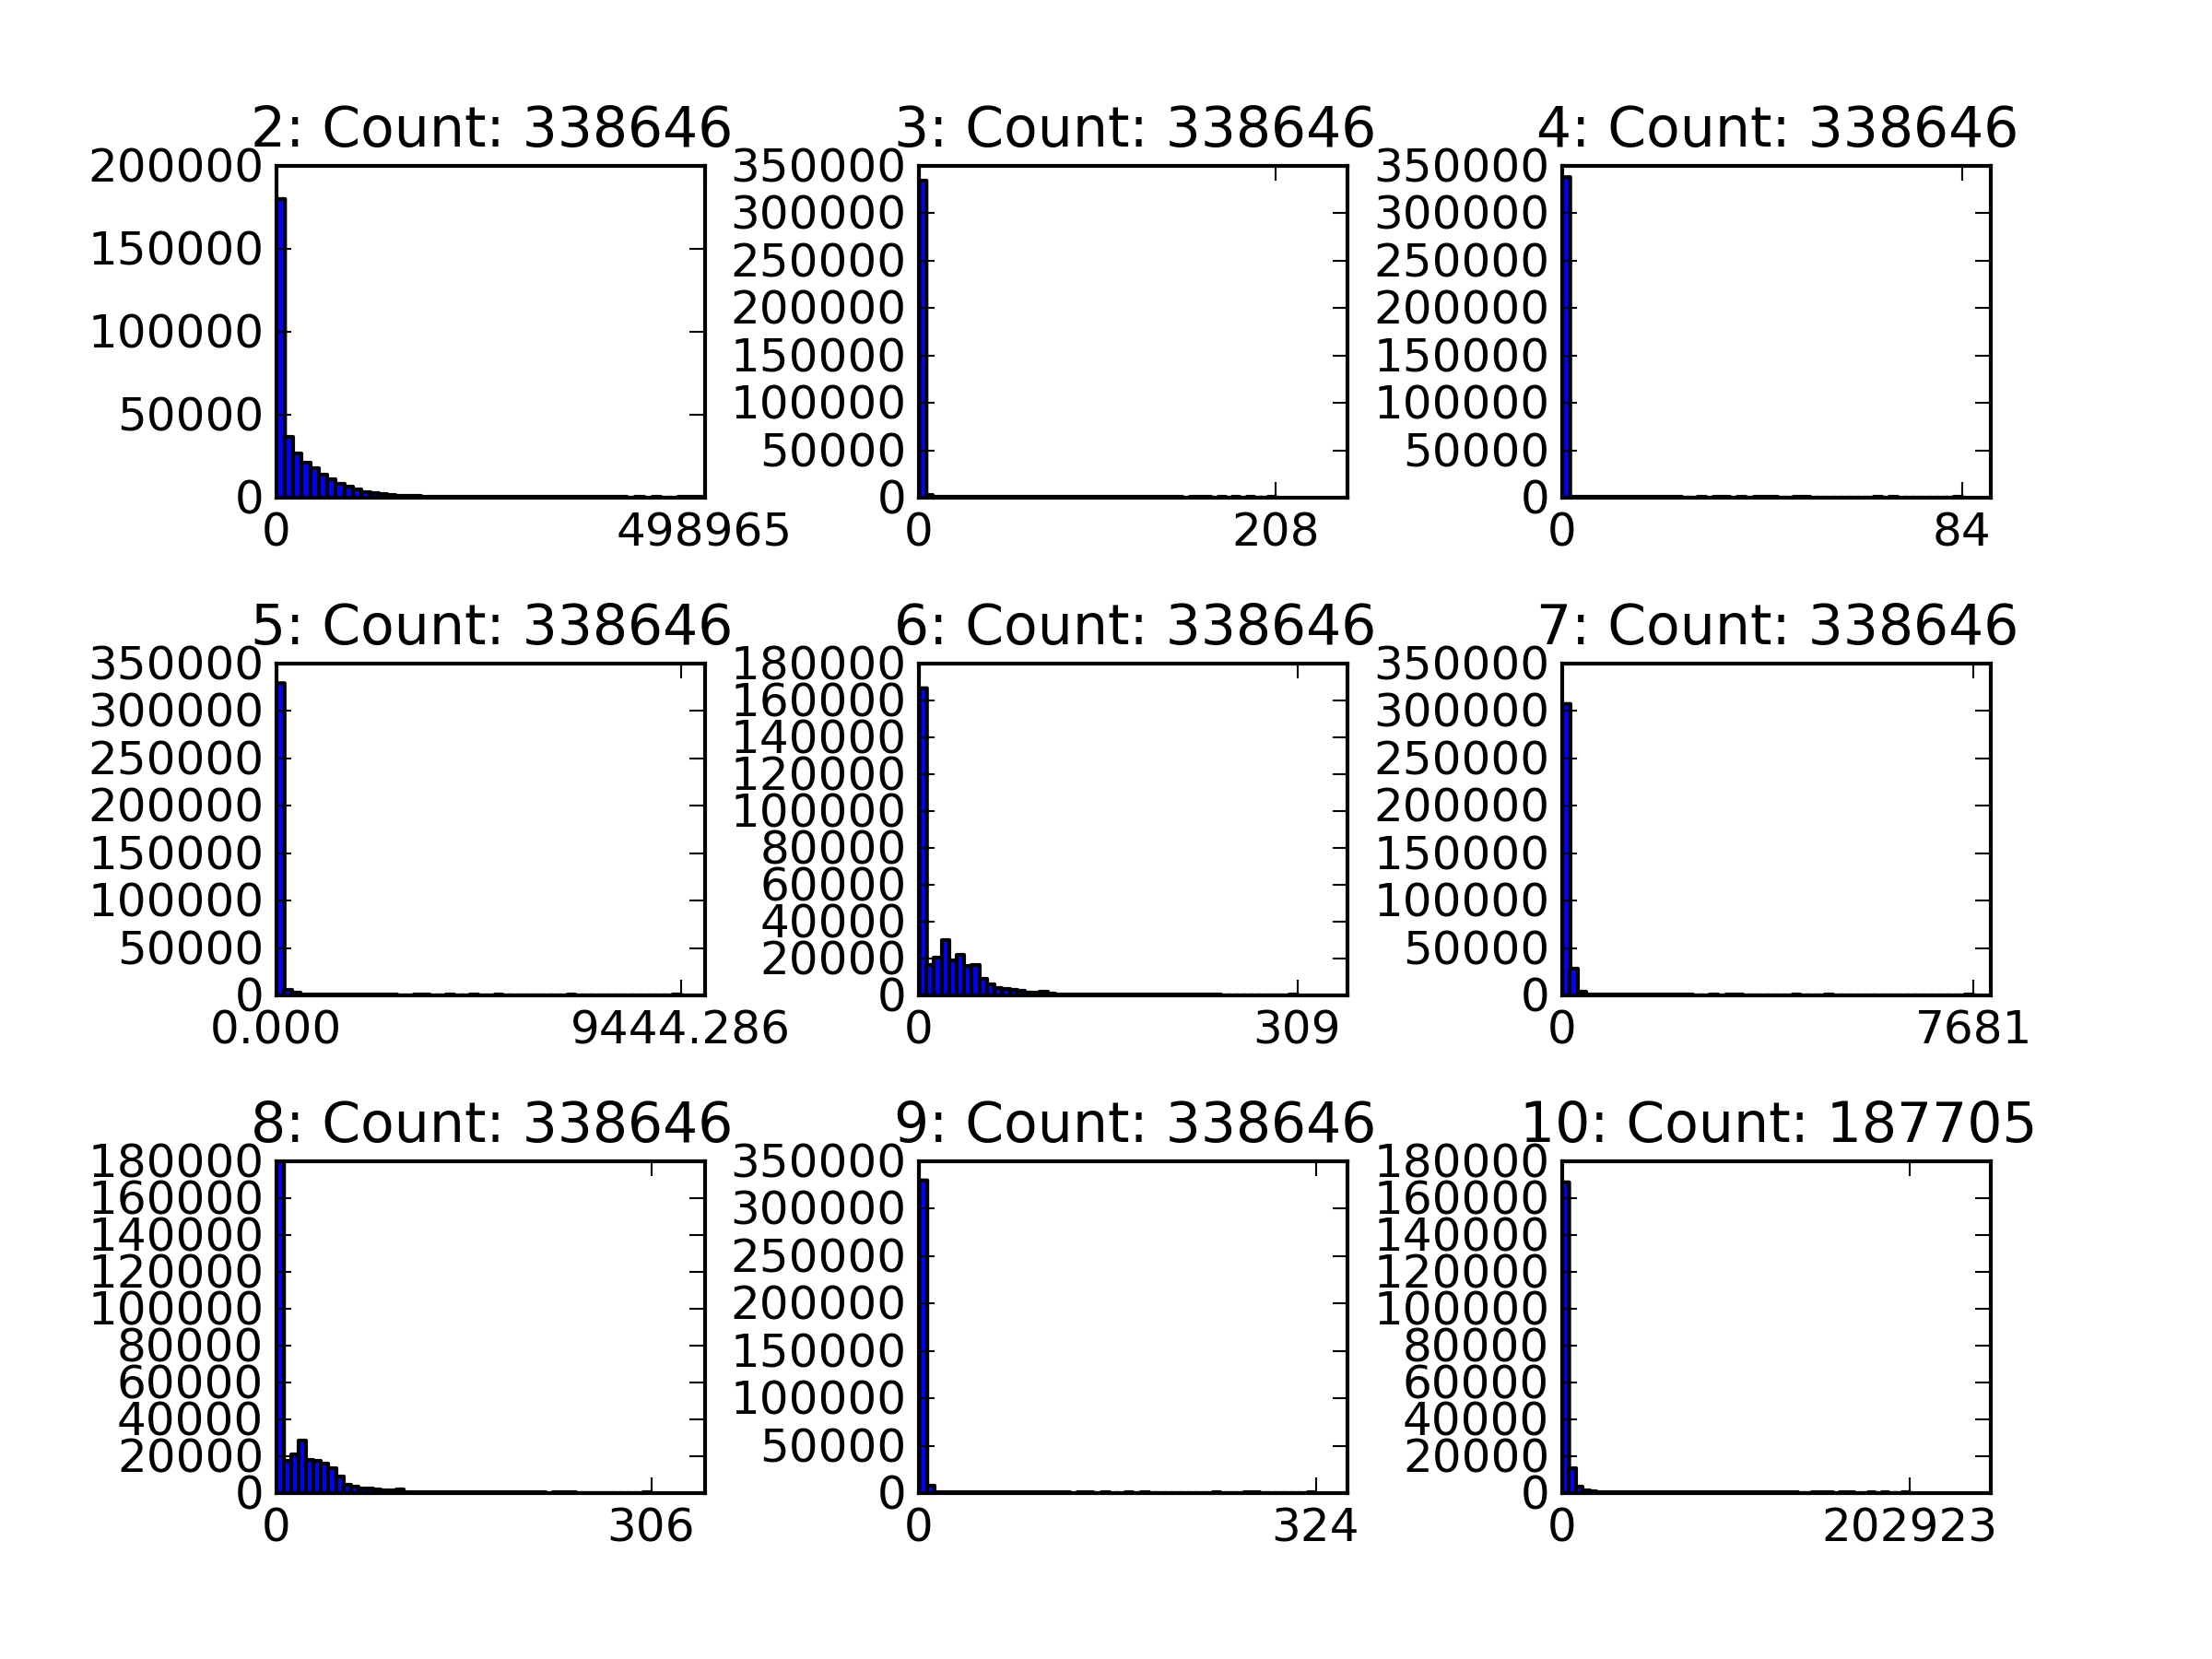
\includegraphics[width=1.0\textwidth]{figures/feature_distributions/features_2_10.png}
\end{figure}

\begin{figure}[ht!]
  \caption{The distribution of feature values for \x{11} through \x{201}}\label{fig:features_11_19}
  \centering
    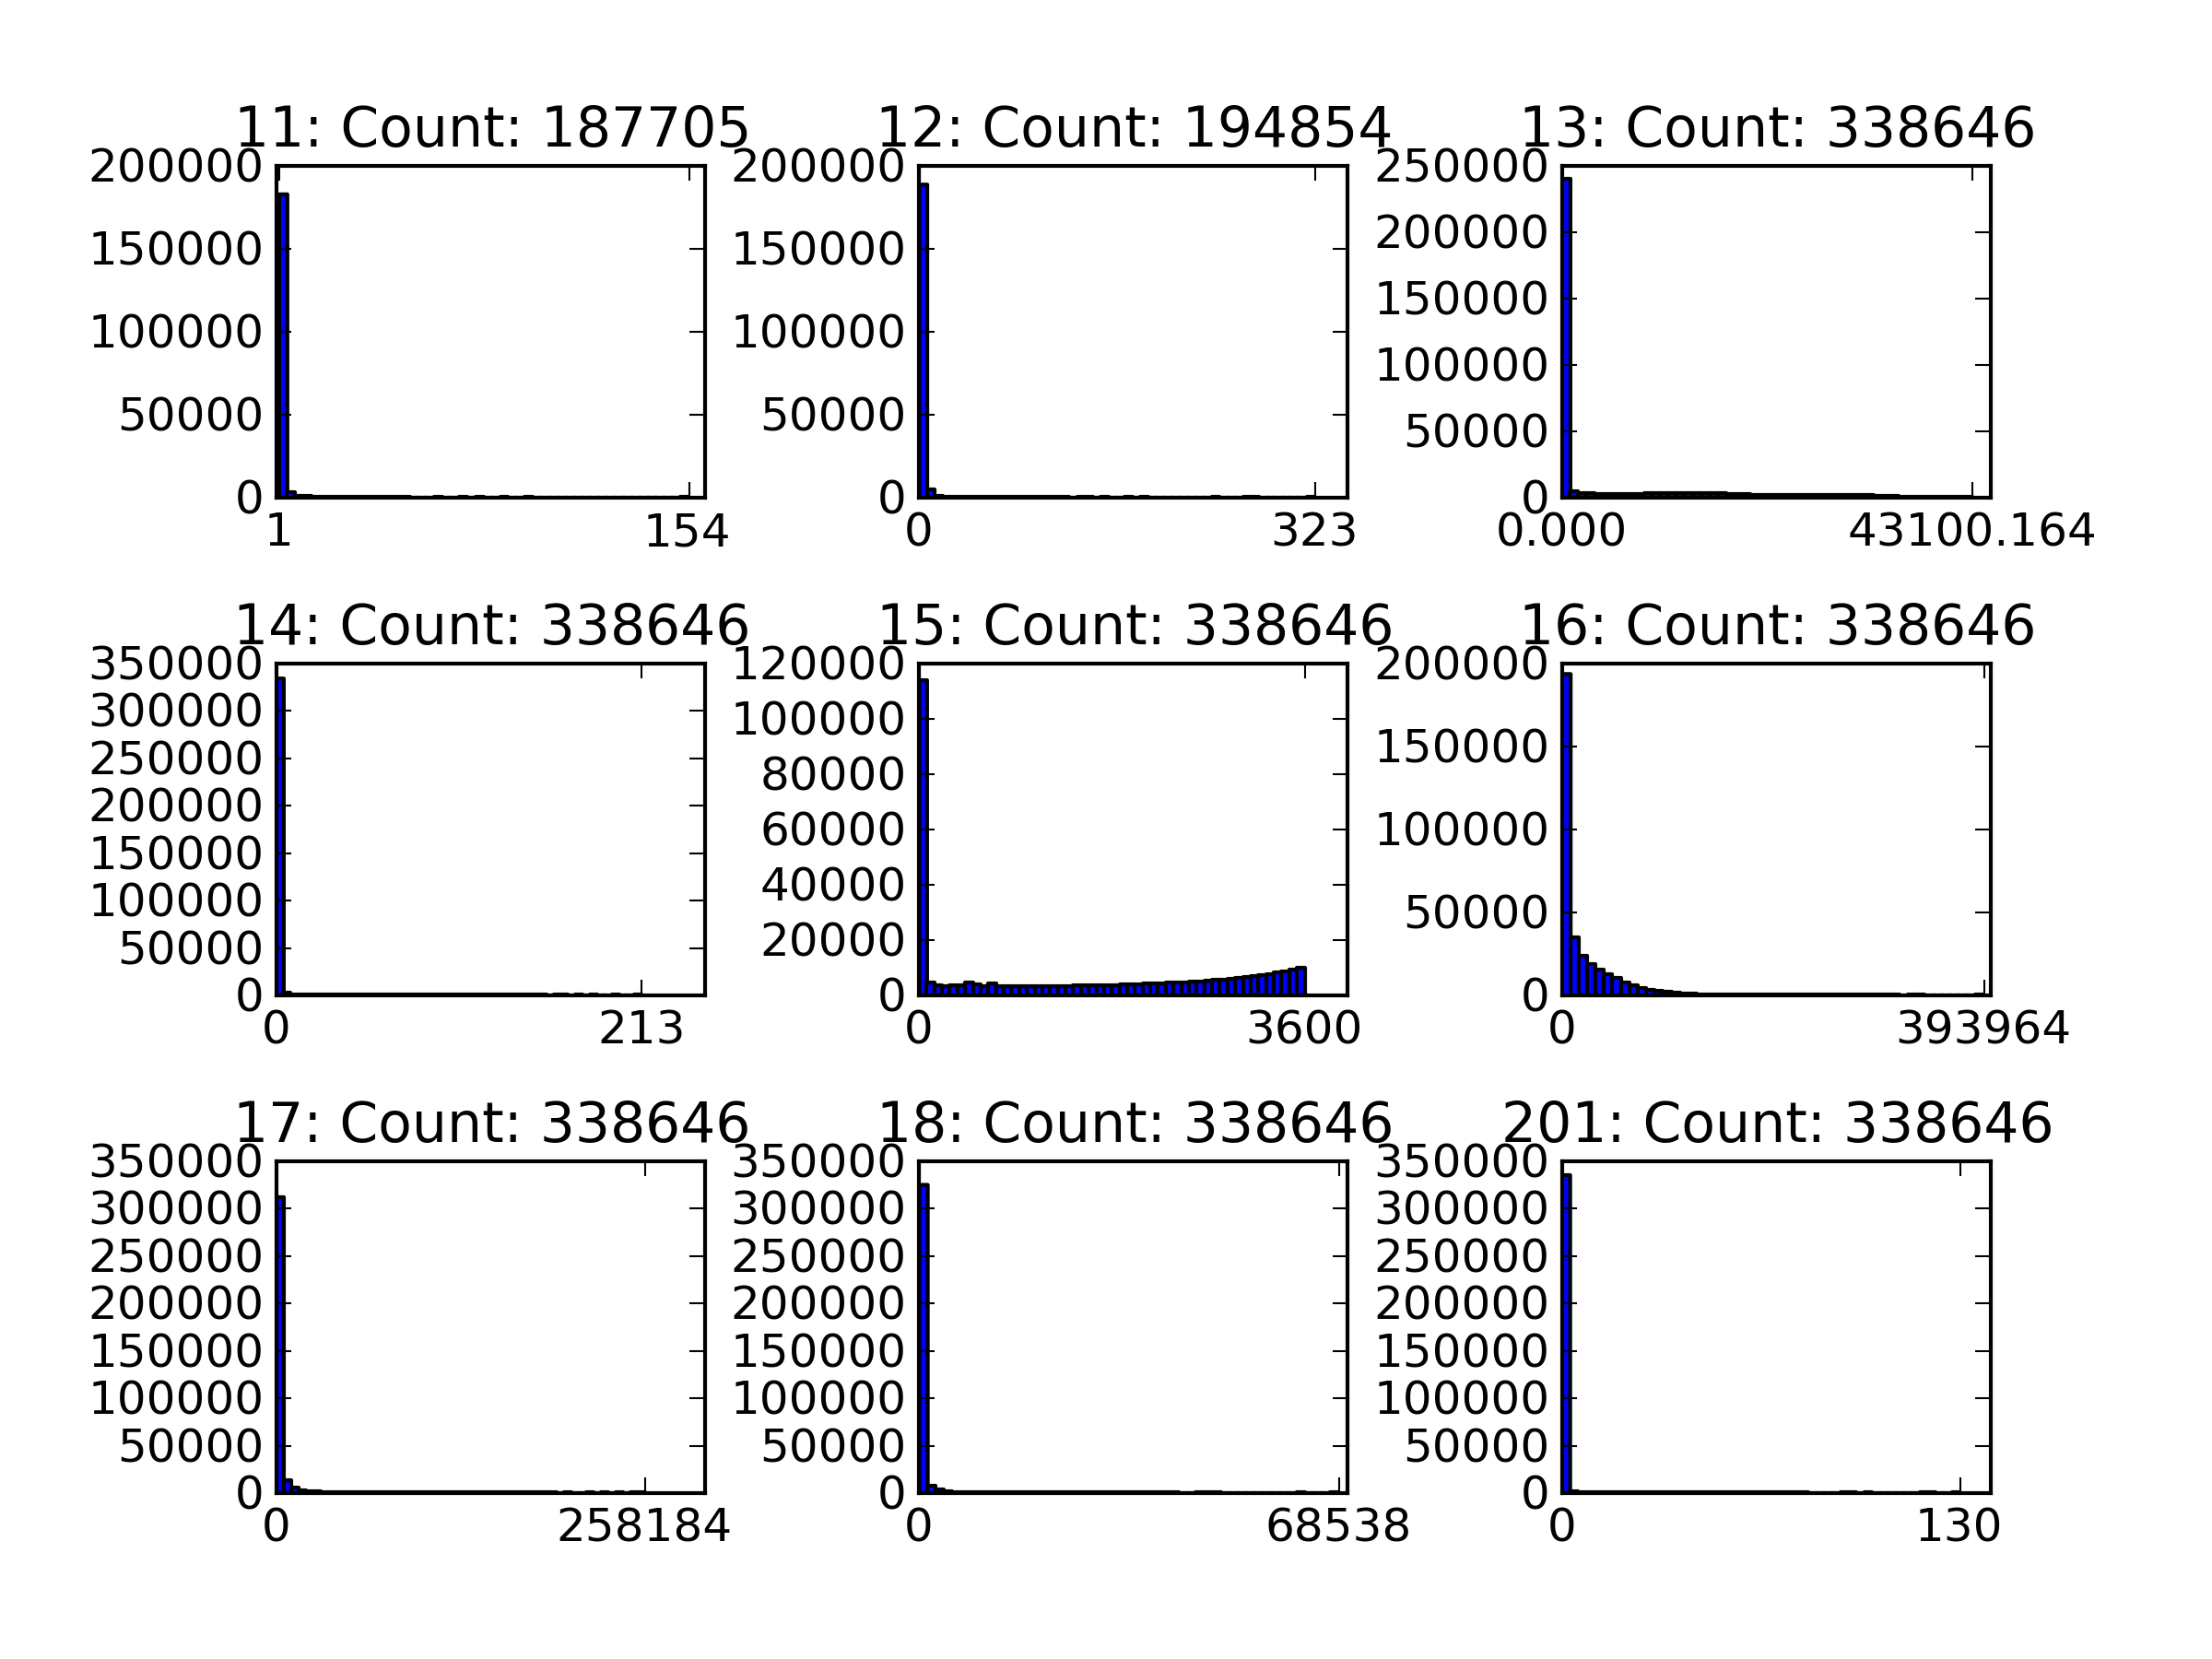
\includegraphics[width=1.0\textwidth]{figures/feature_distributions/features_11_19.png}
\end{figure}

\begin{figure}[ht!]
  \caption{The distribution of feature values for \x{202} through \x{210}}\label{fig:features_20_28}
  \centering
    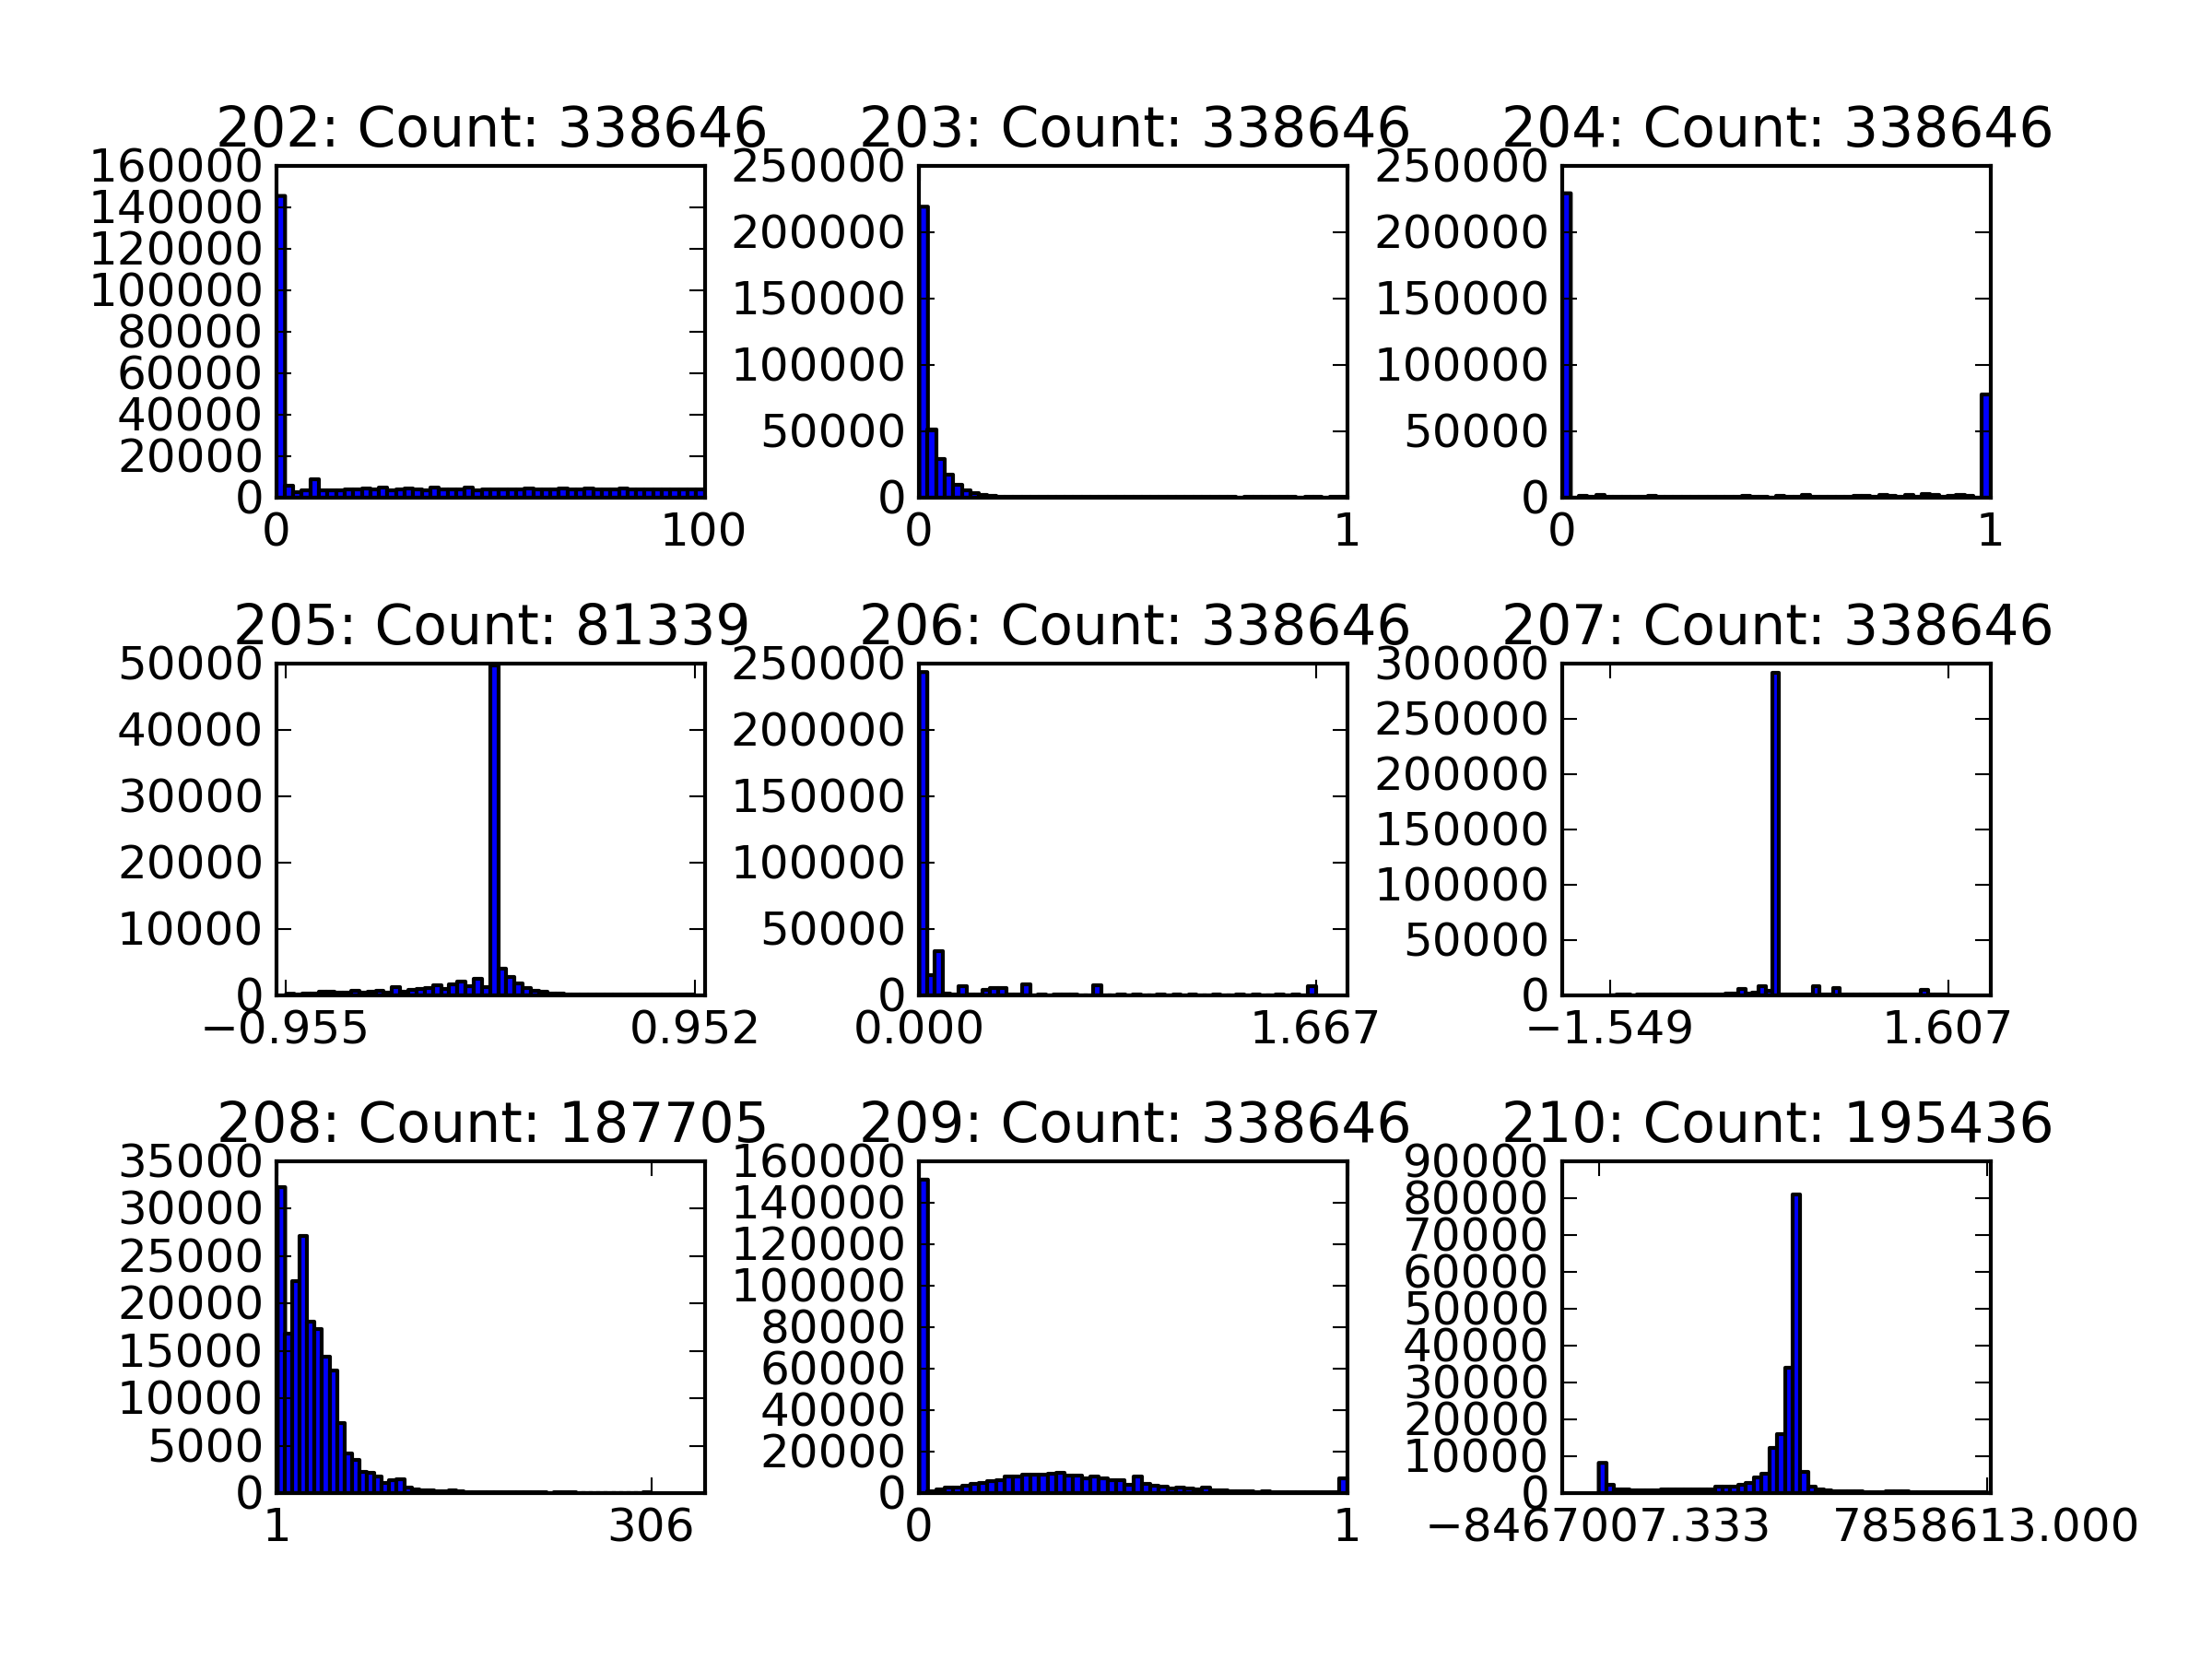
\includegraphics[width=1.0\textwidth]{figures/feature_distributions/features_20_28.png}
\end{figure}

Figures \ref{fig:features_2_10} through \ref{fig:features_20_28} shows the distribution of feature values over every student week where the student was not stopped out. Note that the majority of feature values are 0s. This means there are many weeks where a student did not interact with the course at all, or only interacted with limited course components (for example, never posted on the forum but watched lectures, or only watched lectures but did not submit). Most features are heavily skewed to the right.

\section{Principal Component Analysis}
We performed a dimensionality reduction technique called principal component analysis to transform our extracted features into a basis of lower dimensionality. This technique finds the dimension of the data with the largest variance, and uses this as the first basis dimension. The second basis dimension is the dimension orthogonal to the first which has the largest variance. This process is completed until a full basis is found. The first X dimensions that cover 95\% of the variance are used to transform the features. We use the transformed features as a new dataset. This process not only reduces the dimensionality, but is useful for models that assume feature independence as the PCA features are orthogonal.

Principal component analysis reduced the \neither and \forum cohorts from 28 features to 9 features. PCA transformed the \both cohort into 13 features. We were unable to perform PCA on the \wiki cohort because there were too few students.

\section{Discretization of features}\label{section:binning}
We discretized the extracted feature values as some of our predictive modelling training algorithms rely on discretized values for tractability. This process is also known as ‘binning.’ In order to best discretize a feature, we want to preserve as closely as possibly the distribution of that feature. Inevitably, because we have a smaller range of values than the feature can take, we will lose information when we bin the features, but a good discretization preserves as much information as possible. 
A simple way to bin a continuously valued feature is to use equal sized bins, which works well when the distribution is roughly equally distributed. However, after analyzing our distributions, we realized that our distribution for most features is heavily skewed towards 0. We used a binning strategy that picked binning cutoffs in order to create an equal frequency of samples in each bin. This strategy, as closely as possible, will preserve the original distribution.
We attempted binning with 5 bins and 10 bins. After the binning, we analyzed the distribution of each discretized feature in comparison with the continuous distribution. With just 5 bins, we were able to get almost equal bin frequencies. (see Figures \ref{fig:features_bin_5_2_10} through \ref{fig:features_bin_5_20_28}). Since the distribution roughly captured the entropy, we decided to use 5 bins. Additionally, we knew from prior experiments that a smaller number of bins significantly reduced training and inference times for dynamic Bayesian networks.

\begin{figure}[ht!]
  \caption{The distribution of binned feature values for \x{2} through \x{10}}\label{fig:features_bin_5_2_10}
  \centering
    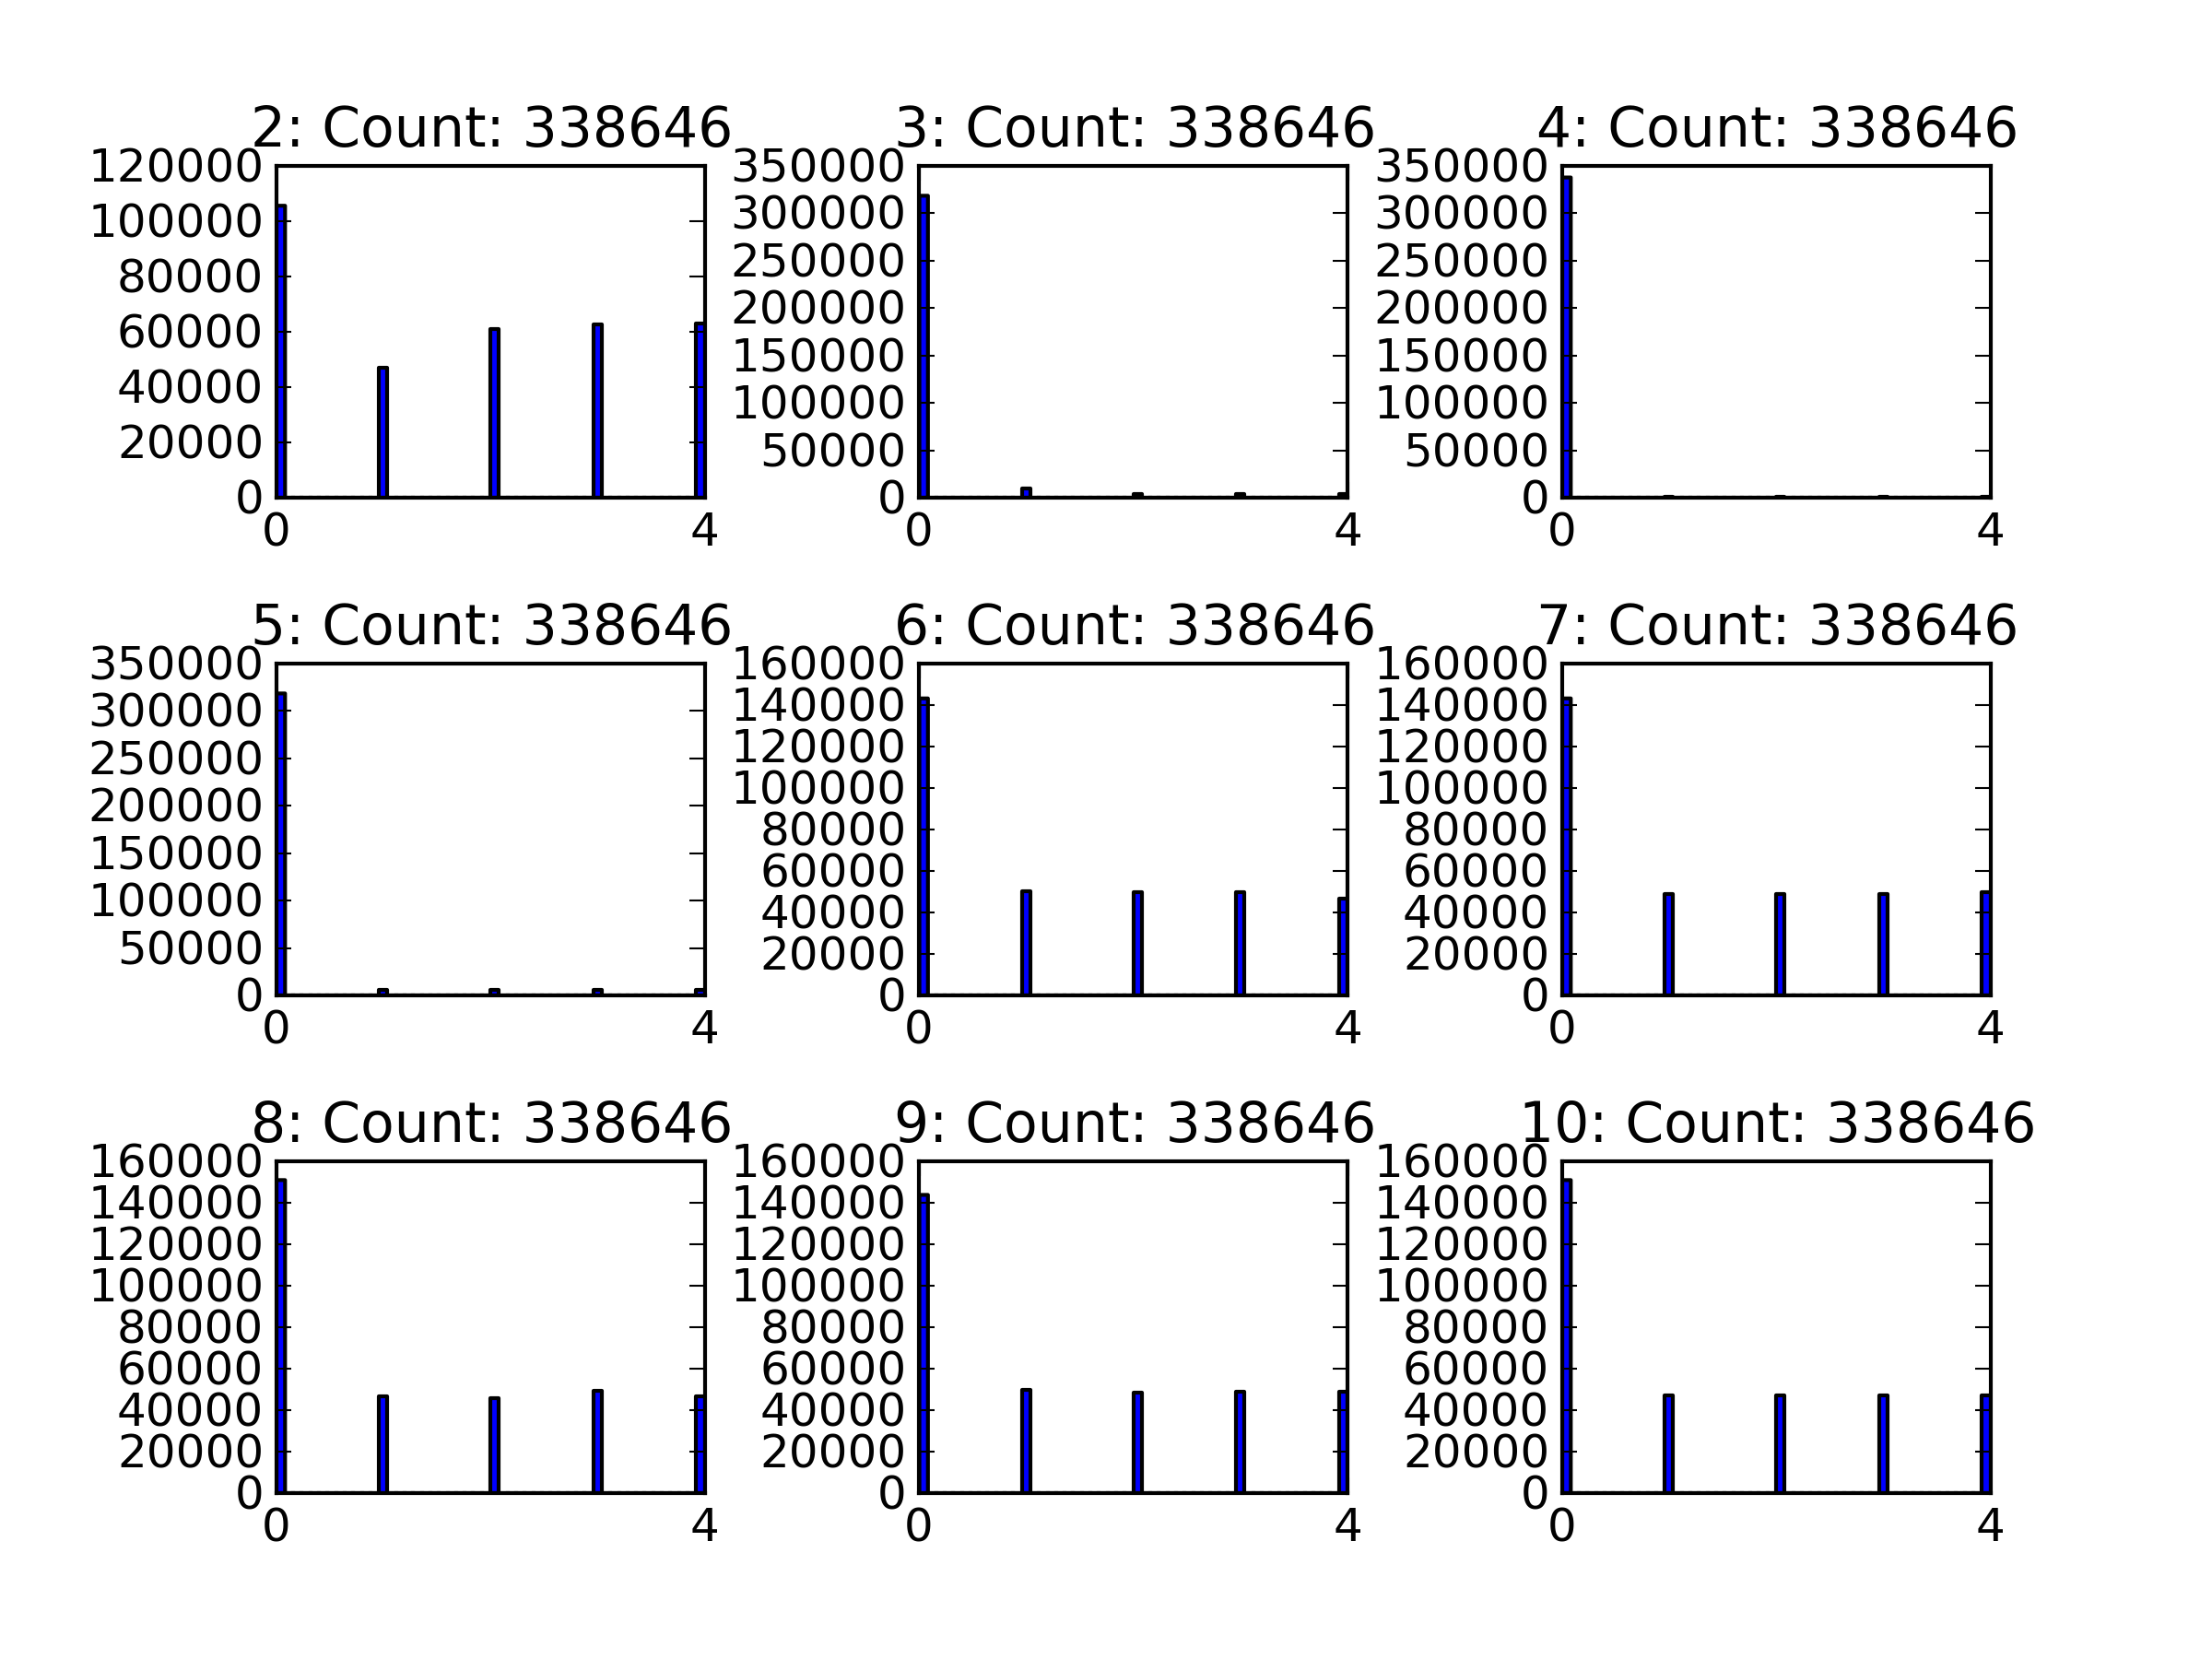
\includegraphics[width=1.0\textwidth]{figures/feature_distributions/features_bin_5_2_10.png}
\end{figure}

\begin{figure}[ht!]
  \caption{The distribution of binned feature values for \x{11} through \x{201}}\label{fig:features_bin_5_11_19}
  \centering
    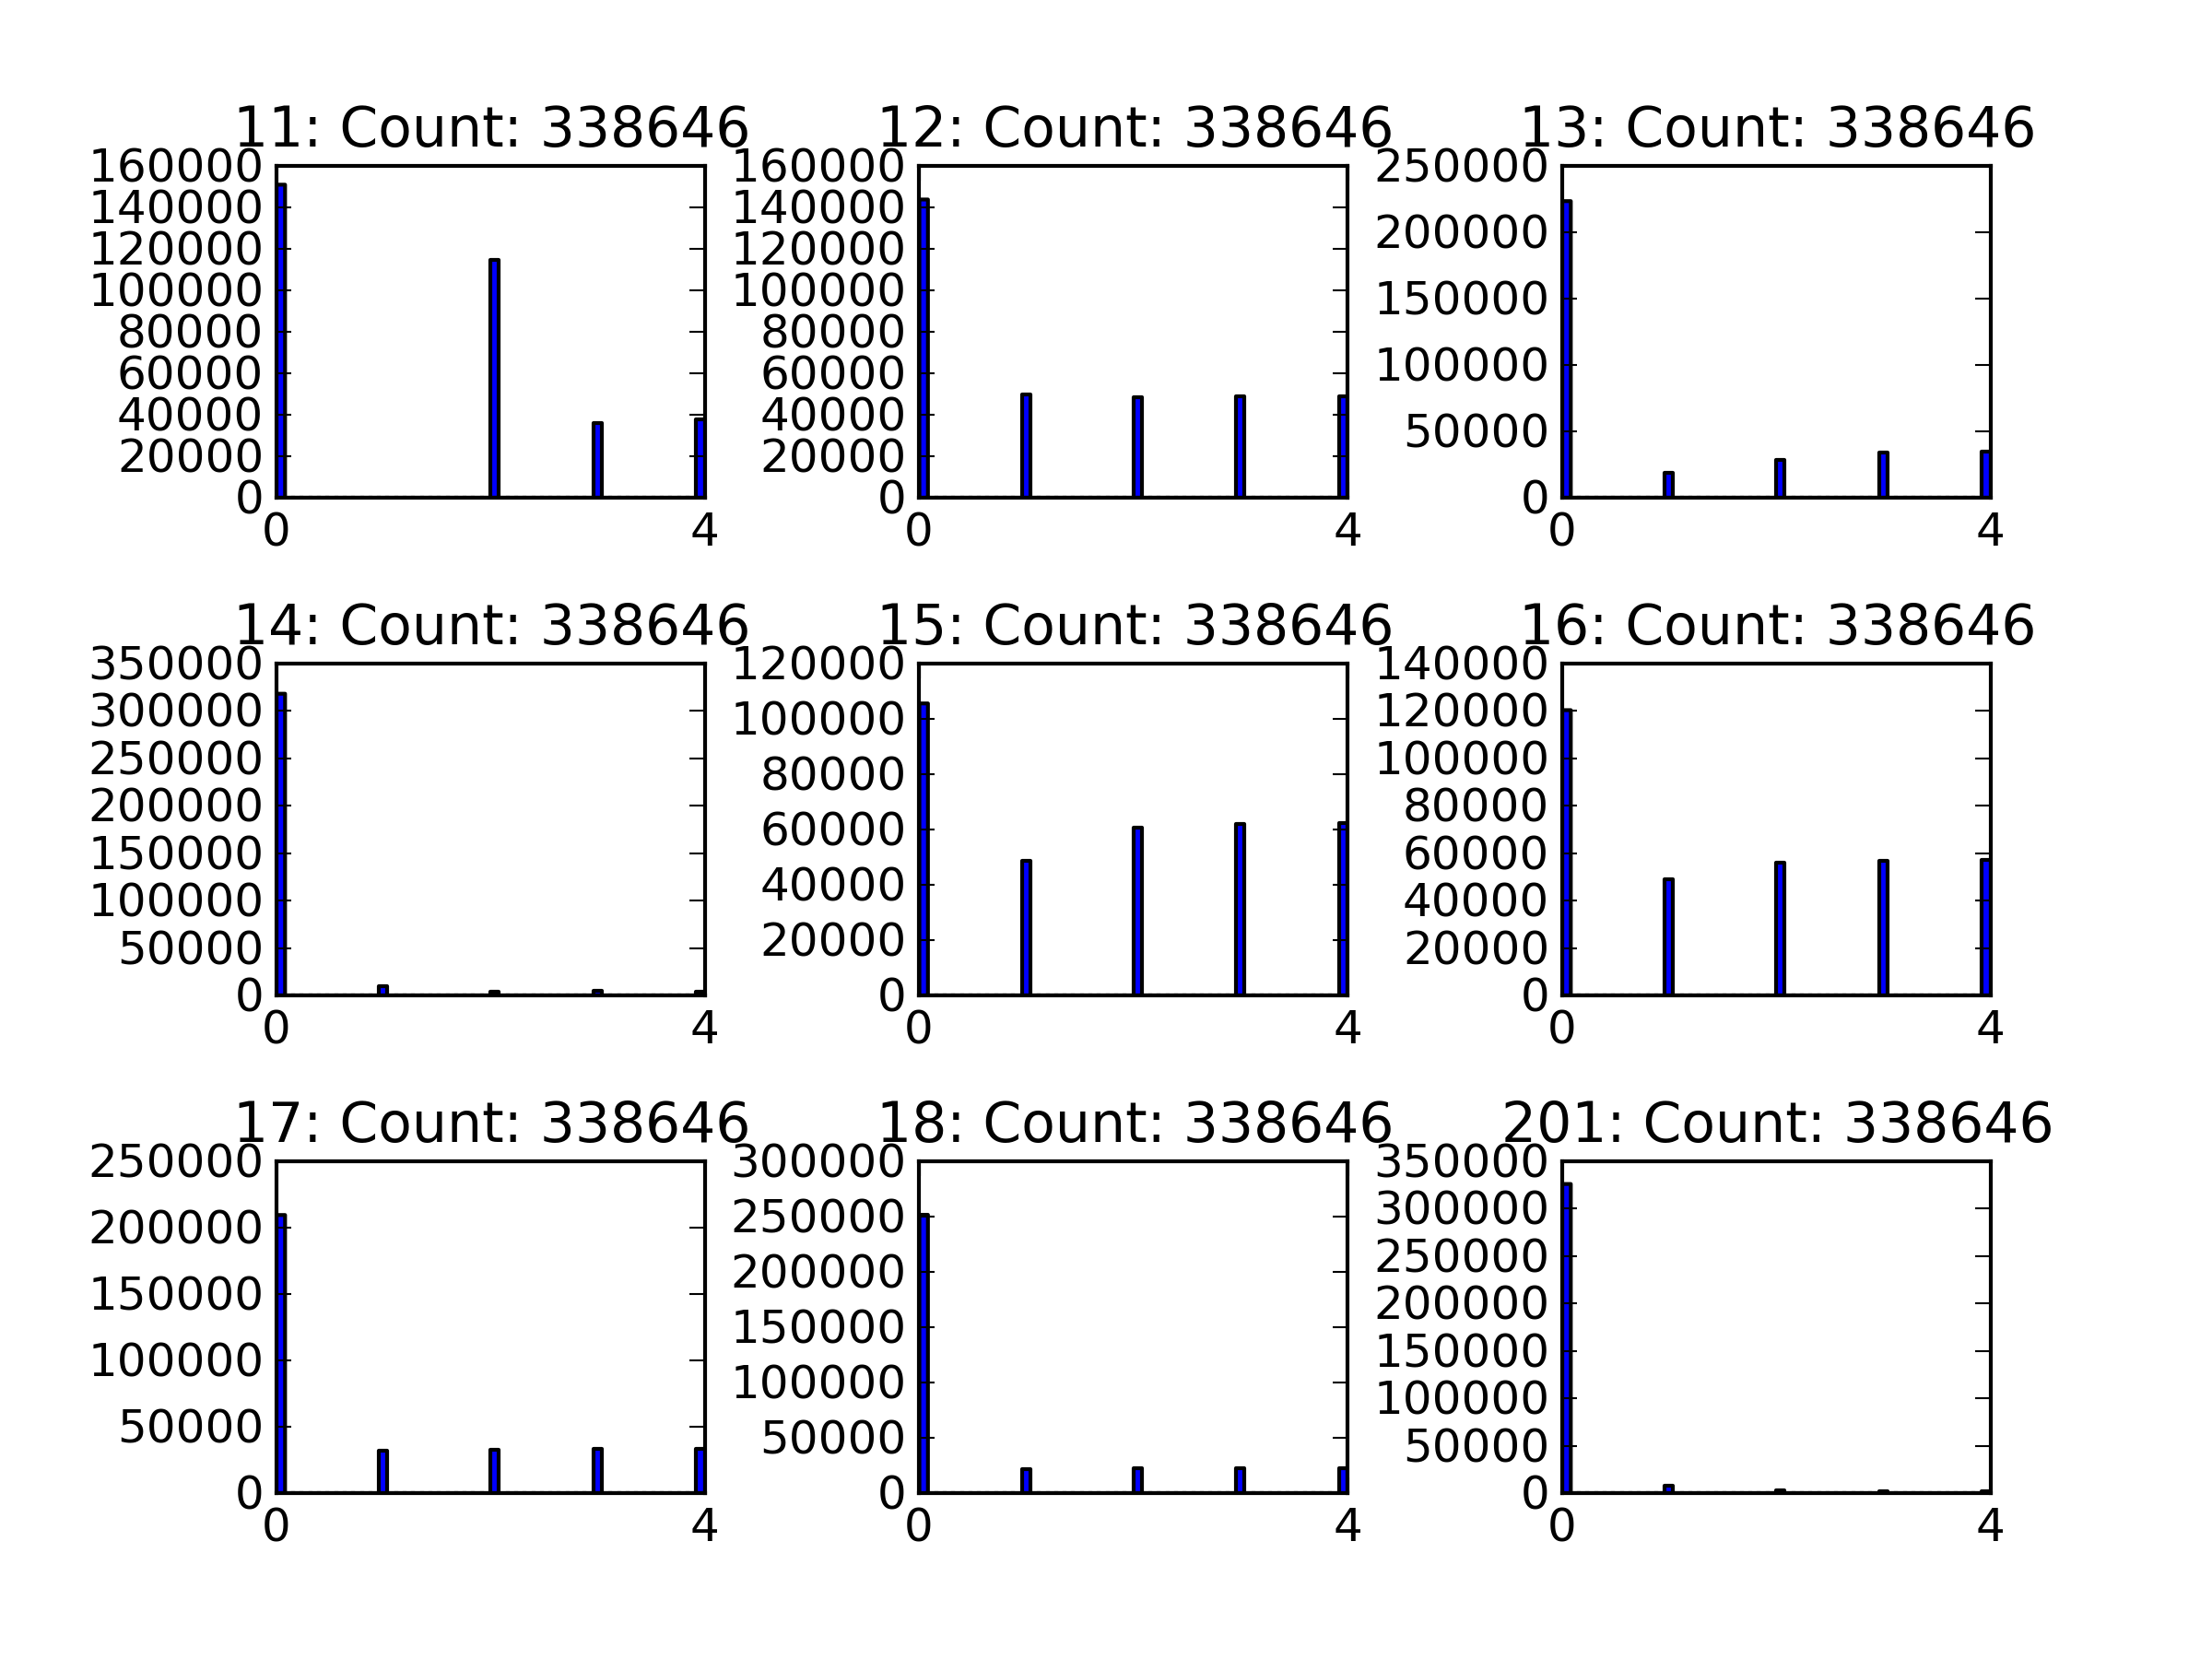
\includegraphics[width=1.0\textwidth]{figures/feature_distributions/features_bin_5_11_19.png}
\end{figure}

\begin{figure}[ht!]
  \caption{The distribution of binned feature values for \x{202} through \x{210}}\label{fig:features_bin_5_20_28}
  \centering
    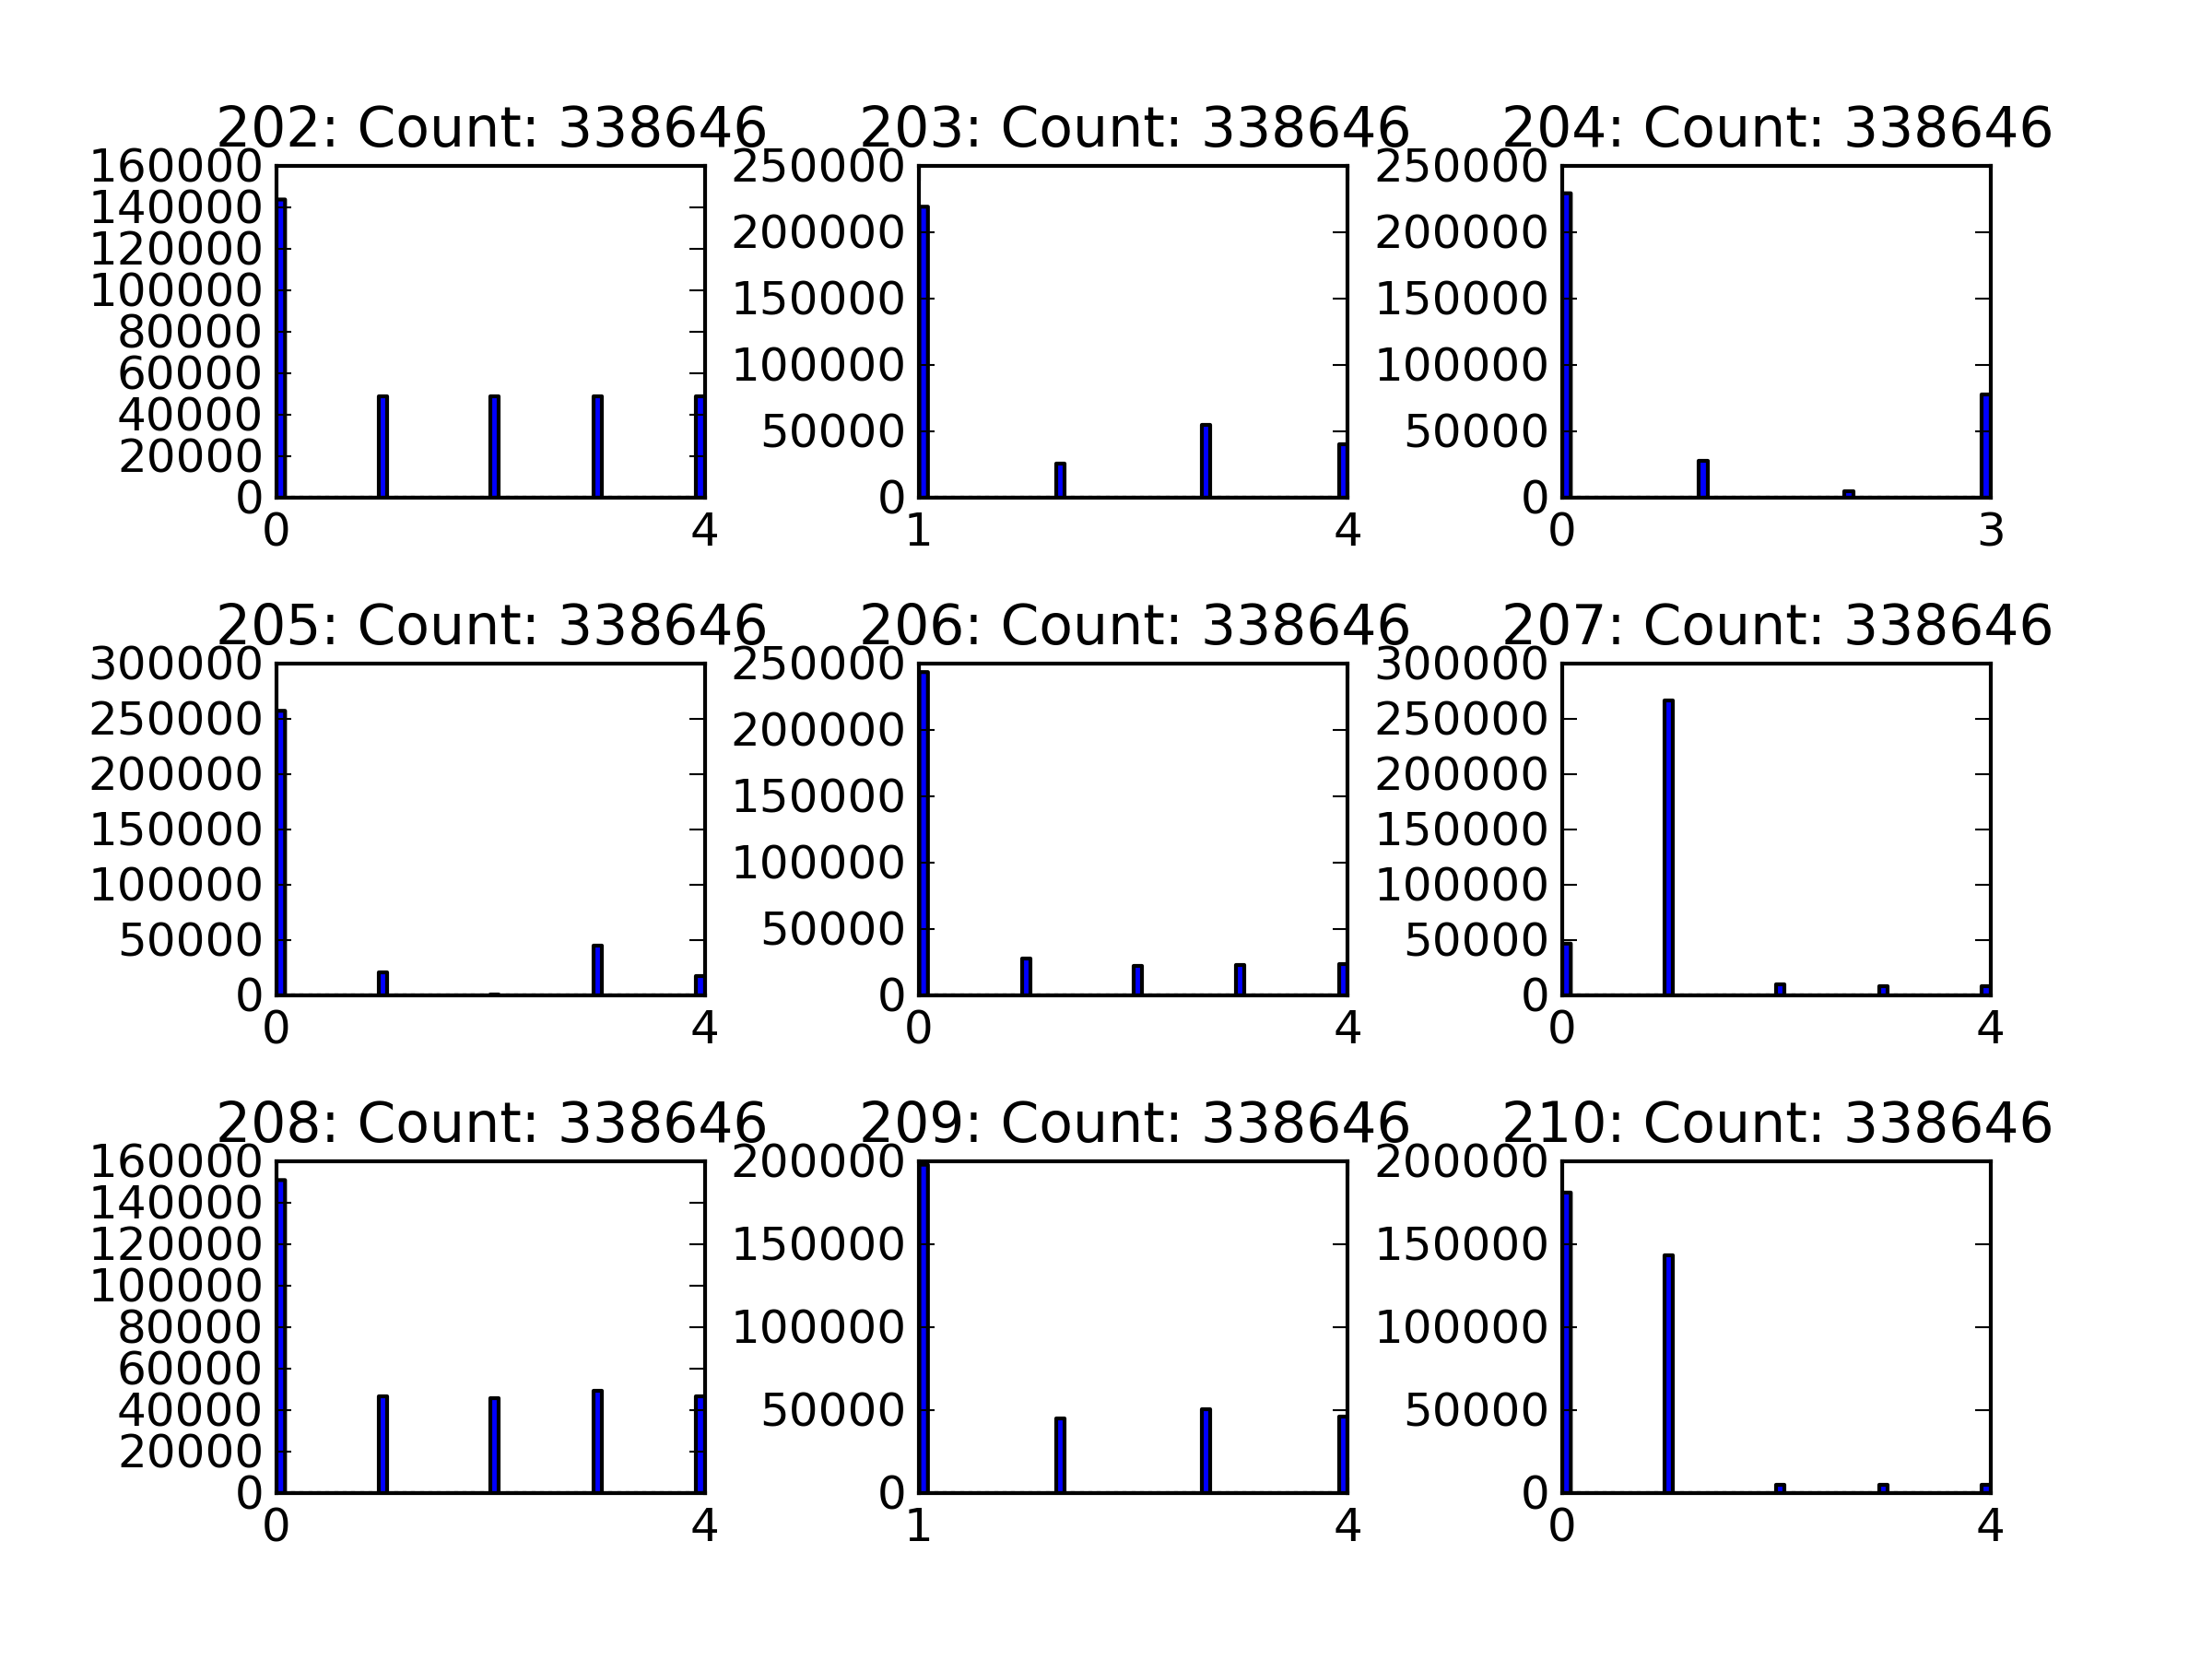
\includegraphics[width=1.0\textwidth]{figures/feature_distributions/features_bin_5_20_28.png}
\end{figure}
